\documentclass{article}

\usepackage[french]{babel}
\usepackage[T1]{fontenc}
\usepackage[letterpaper,top=2cm,bottom=2cm,left=3cm,right=3cm,marginparwidth=1.75cm]{geometry}
\usepackage{amsmath}
\usepackage{graphicx}
\usepackage{enumitem}
\usepackage{subfig}
\usepackage{float}
\usepackage{array}
\usepackage{longtable}
\usepackage{fancyhdr}
\usepackage{listings}
\usepackage{xcolor}

\usepackage{booktabs}
\usepackage{tabularx}

% ========= TCOLOR BOX DEF ========= %
\usepackage[most]{tcolorbox}
\tcbset{
  colback=gray!5,
  colframe=gray!50,
  boxrule=0.5pt,
  arc=2mm,
  left=8pt,right=8pt,top=2pt,bottom=2pt,
  fonttitle=\bfseries
}
\newtcolorbox{resultbox}[1]{title={#1}}
% ================================== %


% ========= YALCC COLOR FOR CODE ========= %
\definecolor{keywordcolor}{RGB}{0,0,180}
\definecolor{commentcolor}{RGB}{100,100,100}
\definecolor{stringcolor}{RGB}{163,21,21}
\definecolor{identifiercolor}{RGB}{10,80,10}
\lstdefinelanguage{YaLCC}{
  morekeywords={Prog,Is,End,If,Then,Else,While,Do,Input,Print},
  morecomment=[l]{\$},      % single-line comments
  morecomment=[s]{!!}{!!},  % long comments
  morestring=[b]",           % string-like constructs if needed
  sensitive=true             % case-sensitive
}
\lstdefinestyle{yalccstyle}{
  language=YaLCC,
  basicstyle=\ttfamily\small,
  keywordstyle=\color{keywordcolor}\bfseries,
  commentstyle=\color{commentcolor}\itshape,
  stringstyle=\color{stringcolor},
  identifierstyle=\color{identifiercolor},
  numbers=left,
  numberstyle=\tiny\color{gray},
  stepnumber=1,
  numbersep=6pt,
  frame=single,
  breaklines=true,
  showstringspaces=false,
  tabsize=4
}
% ======================================== %



\pagestyle{fancy}

\fancyhf{}
\fancyhead[L]{\textbf{INFO—F-403 : YaLCC Compiler Project}}
\fancyhead[R]{\textbf{Berthion Antoine, Bontridder Milan}}
\fancyfoot[C]{\thepage}

\usepackage[colorlinks=true, allcolors=blue]{hyperref}

\title{\textbf{INFO—F-403} \\
Introduction to language theory and compiling \\ 
Project Report}
\author{Berthion Antoine - 566199 \and Bontridder Milan - 493709}
\date{15 October 2025}

\begin{document}

\maketitle

\vspace{-2em}

\begin{figure}[H]
    \centering
    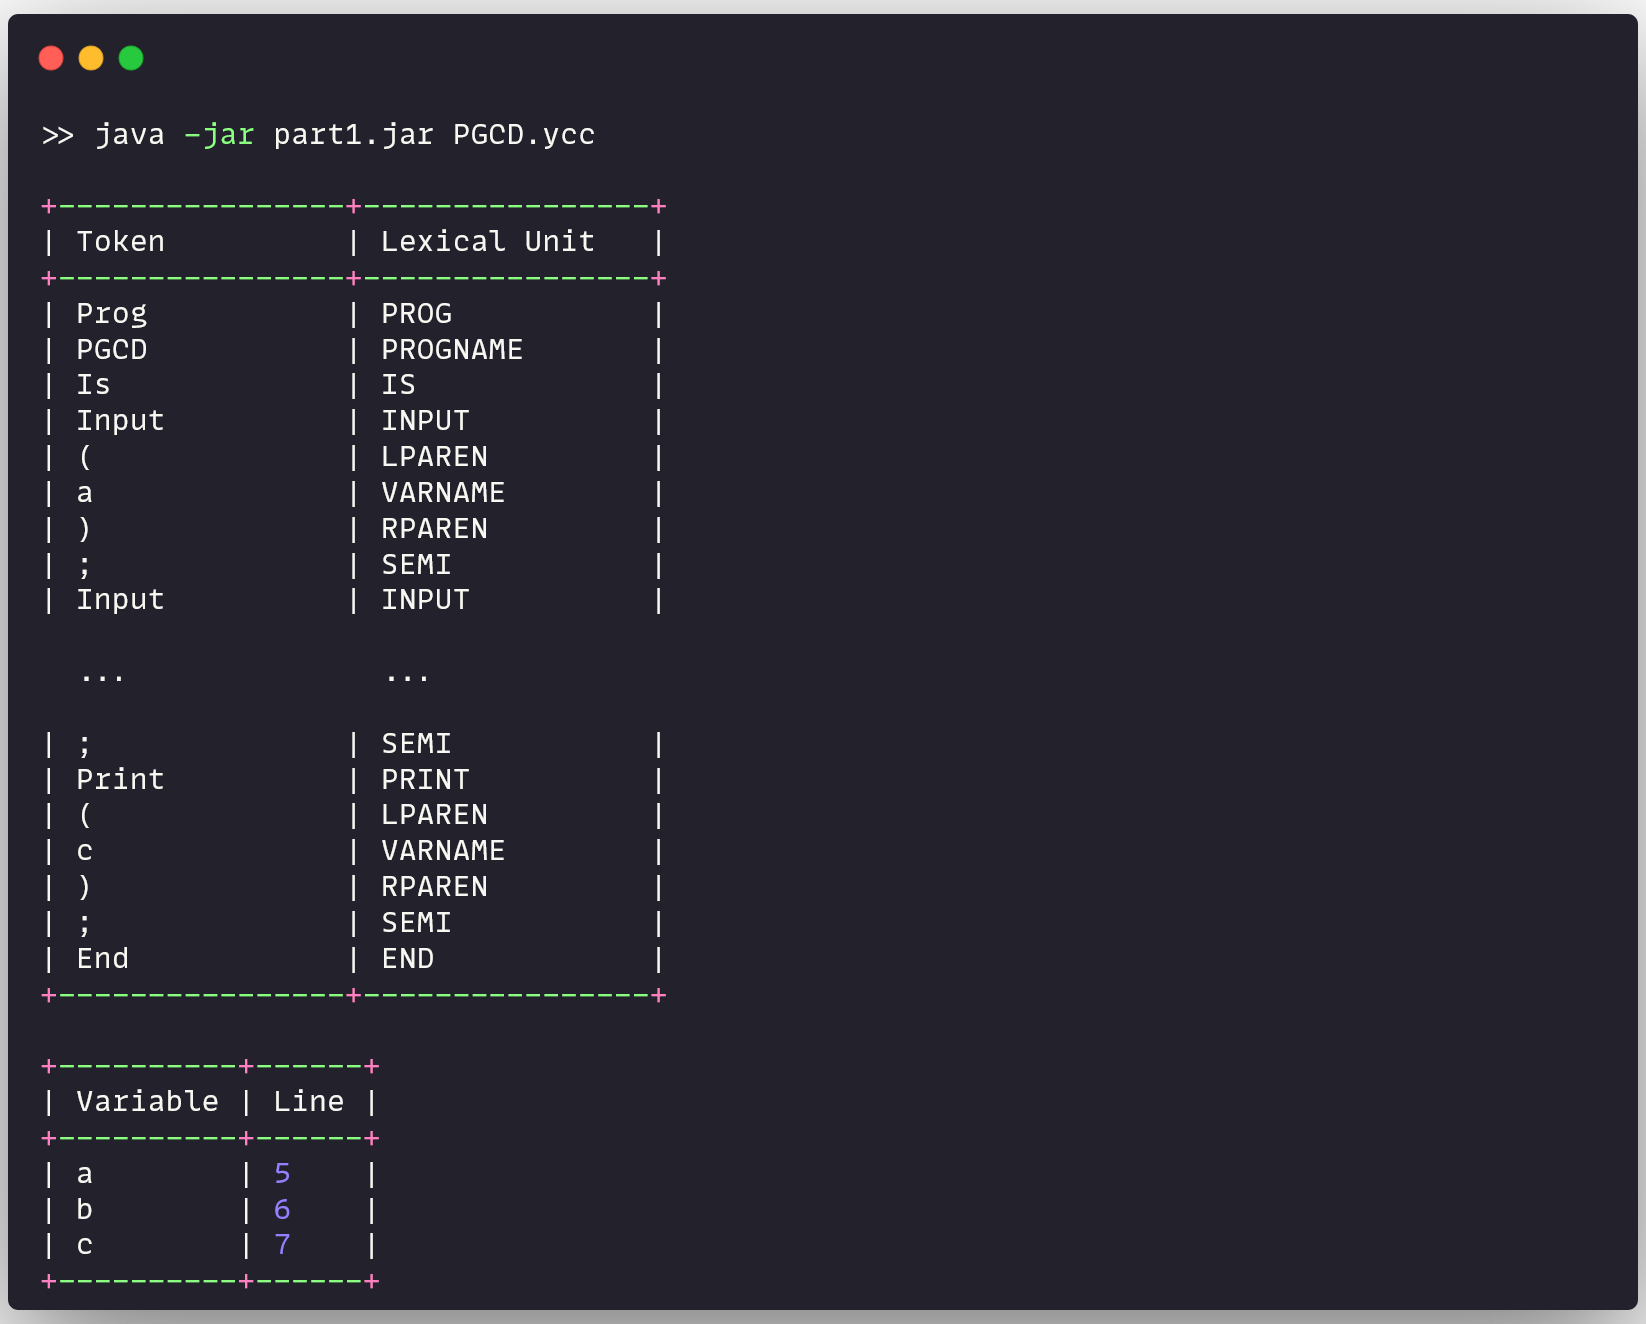
\includegraphics[width=0.7\textwidth]{src/intro.png}
    \label{fig:intro}
    % \caption{...}
\end{figure}

\vspace{-1em}

\section*{Abstract}

This project implements the \textbf{lexical analysis phase} of a compiler for the toy language \textbf{YaLCC} (\textit{Yet Another Language for the Compiler Course}). The \textbf{lexer} reads \texttt{source code} files and produces a stream of \textbf{tokens}, which can later be processed by a \textbf{parser}. This report details the \textbf{design and implementation} of the lexer, the \textbf{regular expressions} used for token recognition, example \texttt{input} and \texttt{output} files, and the \textbf{testing strategy}.


\section{Introduction}

\noindent The \textbf{YaLCC lexer} transforms \texttt{source code} into a well-defined sequence of \textbf{tokens}, accurately identifying \textbf{keywords}, \textbf{variable names}, \textbf{numerical constants}, \textbf{operators}, and \textbf{comments}. The objective of the \textbf{lexical analysis phase} is to systematically recognize and classify the fundamental units of the program that are relevant to the compiler. \\

\noindent Conceptually, the lexer functions as a \textit{"spelling checker"}, ensuring that the individual elements of the code are correctly identified. Subsequently, the \textbf{parser} serves as a \textit{"grammar checker"}, verifying whether these tokens are syntactically arranged to form meaningful constructs according to the rules of the language. \\ \\

\noindent The \textbf{YaLCC language} provides the following features:
\begin{itemize}
    \item Program declarations using \texttt{Prog [ProgName] Is ... End}
    \item Variable declarations and assignments, allowing the definition of identifiers for storing values
    \item Basic arithmetic expressions and operators (\texttt{+}, \texttt{-}, \texttt{*}, \texttt{/})
    \item Conditional statements (\texttt{If ... Then ... Else ... End})
    \item Loops (\texttt{While ... Do ... End})
    \item Input and output statements (\texttt{Input(...)} and \texttt{Print(...)})
    \item Short (\texttt{\$}) and long (\texttt{!!}) comments, which are ignored by the parser \\
\end{itemize}

\noindent The complete \textbf{symbol table}, listing all recognized tokens, is provided in \textbf{Appendix~\ref{appendix:symbol-table}}.


\section{Project Overview}

\noindent The project is organized as follows:

\begin{itemize}
    \item \textbf{\texttt{src/}} : Contains all source files necessary for the \textbf{lexer implementation}, including \texttt{LexicalAnalyzer.flex}, the generated \texttt{LexicalAnalyzer.java}, \texttt{Symbol.java}, \texttt{LexicalUnit.java}, and \texttt{Main.java}.
    \item \textbf{\texttt{doc/}} : Contains the \textbf{Javadoc documentation} and this report PDF.
    \item \textbf{\texttt{test/}} : Contains example \textbf{YaLCC source files} and unit tests implemented using \textbf{JUnit}.
    \item \textbf{\texttt{dist/}} : Contains the executable JAR file \texttt{part1.jar}.
    \item \textbf{\texttt{more/}} : Contains other supporting files, including the project specification document.
\end{itemize}

\noindent The main \textbf{workflow} of the project can be summarized as: \\[6pt]
\begin{center}
\texttt{YaLCC source file (.ycc) → LexicalAnalyzer → sequence of lexical tokens → symbol table}
\end{center}


\section{Regular Expressions}

\noindent The \textbf{lexer} is implemented using \textbf{JFlex}, which generates a \textbf{nondeterministic finite automaton (NFA)} responsible for accepting valid \textbf{tokens} and rejecting invalid ones, while associating each accepted token with its corresponding \textbf{lexical unit} for subsequent processing by the \textbf{parser}. The NFA is then converted into a \textbf{deterministic finite automaton (DFA)} and optimized to minimize the number of states\footnote{The DFA initially had 63 states and was optimized down to 54 states, improving efficiency during lexical analysis.}, improving \textbf{efficiency} during lexical analysis. \\

\noindent To configure the JFlex-generated DFA, it is necessary to provide a set of \textbf{regular expressions}. These expressions define the patterns of valid \textbf{tokens}—such as \textbf{keywords}, \textbf{identifiers}, \textbf{numbers}, and \textbf{operators}—so that any input not matching one of these patterns is automatically rejected, ensuring that the lexer correctly identifies only the valid \textbf{lexical units}.


\subsection{Specific Tokens (Keywords, Operators, and Symbols)}

\noindent The \textbf{lexer} first identifies \textbf{specific tokens} corresponding to \textbf{reserved keywords}, \textbf{operators}, and \textbf{punctuation}. These are matched literally in the input stream. Examples include:

\begin{itemize}
    \item \texttt{Prog, Is, End} – denote the beginning and end of a \textbf{program}.
    \item \texttt{If, Then, Else} – represent \textbf{conditional statements}.
    \item \texttt{While, Do} – denote \textbf{loops}.
    \item \texttt{Input, Print} – handle \textbf{input/output operations}.
    \item \textbf{Operators and punctuation symbols:} \texttt{+}, \texttt{-}, \texttt{*}, \texttt{/}, \texttt{=}, \texttt{==}, \texttt{<=}, \texttt{<}, \texttt{(}, \texttt{)}, \texttt{;}.
\end{itemize}

\noindent These tokens are recognized by \textbf{exact string matches}, ensuring that reserved words and syntactic symbols are correctly identified before general pattern matching.


\subsection{Pattern-Based Tokens (Identifiers, Numbers, Comments, Whitespace)}

\noindent The following regular expressions are used to recognize variable identifiers, numbers, comments, and whitespace:

\begin{itemize}

    \item \texttt{ID\_PROG = [A-Z][A-Za-z0-9\_]*} \\
    Matches program identifiers that start with an uppercase letter followed by any combination (or None) of letters, digits, or underscores. This is case sensitive.
    
    \item \texttt{ID\_VAR = [a-z][A-Za-z0-9\_]*} \\  
    Matches variable identifiers beginning with a lowercase letter, followed by letters, digits, or underscores. This enforces case sensitivity and distinguishes variables from program identifiers.
    
    \item \texttt{NUMBER = [0-9]+} \\  
    Matches integer constants composed of one or more digits. Only positive integers are considered, and negative numbers are handled via the minus operator rule.
    
    \item \texttt{WHITESPACE = [ \textbackslash t\textbackslash r\textbackslash n]+} \\  
    Matches sequences of spaces, tabs, and newline characters. These are ignored by the lexer and do not produce tokens, as they are not meaningful for the parser.
    
    \item \begin{verbatim}SHORT_COMMENT = \$.* \end{verbatim} 
    Matches short comments starting with a dollar sign and continuing to the end of the line. These are skipped by the lexer and do not contribute to the token stream.
    
    \item \begin{verbatim}LONG_COMMENT = \!\!([^!]|!\+[^!])*?\!\! \end{verbatim}
    Matches long comments enclosed between double exclamation marks. The pattern allows any content that does not include the closing \texttt{!!}, ensuring that nested comments are not accepted, as per the language specification.
    
\end{itemize}

\noindent Together, these regular expressions ensure that the lexer can accurately identify all valid lexical units while ignoring irrelevant or non-semantic content.

\section{Lexer Design and Implementation}

\noindent The \textbf{YaLCC lexer} is implemented in \textbf{Java} using \textbf{JFlex}. The core definition resides in \texttt{LexicalAnalyzer.flex}, which specifies the \textbf{regular expressions} and the corresponding actions executed for each matched \textbf{token}. \\

\noindent Upon recognizing a token, the lexer constructs a \texttt{Symbol} object containing the \textbf{token text}, its \textbf{lexical unit}, and its \textbf{position} (line and column) within the \texttt{source file}. These \textbf{Symbol} objects are then sequentially passed to the \textbf{parser} for \textbf{syntactic analysis}. \\

\noindent Key \textbf{design considerations} include:

\begin{itemize}
    \item \textbf{Modular Token Representation:} Each \textbf{lexical unit} is encapsulated in a \texttt{Symbol} object, ensuring a consistent interface between the lexer and parser.
    \item \textbf{Error Handling:} Unrecognized or invalid characters trigger immediate error messages to \texttt{System.err}, including the precise location (yy) in the source code, facilitating debugging.
    \item \textbf{Lexer-Parser Integration:} Tokens are returned in the order they appear in the \texttt{source file}, preserving \textbf{program structure} and enabling deterministic parsing without ambiguity.
\end{itemize}

\noindent This design ensures the \textbf{lexer} is \textbf{efficient}, \textbf{maintainable}, and \textbf{robust}, providing a solid foundation for the subsequent \textbf{parsing} and \textbf{semantic analysis} phases.


\section{Sample Programs and Lexical Analysis Results}

\noindent To evaluate our \textbf{YaLCC lexer}, we executed it on various \texttt{.ycc} programs to analyze its \textbf{output behavior}. Additionally, we employed \textbf{unit testing} to ensure that our \textbf{lexical analyzer} functioned as intended. For further details on the unit testing methodology, see Section~\ref{section:tests}.  

\noindent Several of the \texttt{.ycc} files used for testing are provided in the \textbf{Appendix~\ref{appendix:example-ycc}}. The primary objective was to observe how the lexer responded to specific situations, including, but not limited to: excessive or irregular whitespace, invalid tokens, extensive long comments, syntactically incorrect code, and complex sequences of tokens.


\section{Lexer Verification via Unit Tests}
\label{section:tests}

\noindent The lexical analyzer has been rigorously tested using \textbf{JUnit 5}. The test suite is designed to verify that the lexer correctly identifies tokens, handles errors, and maintains a consistent symbol table. Key aspects of the testing strategy include:

\begin{itemize}
    \item \textbf{Lexical Unit Validation:} Tests confirm that each token is correctly classified as a keyword, identifier, number, operator, or punctuation symbol, ensuring accurate token recognition.
    \item \textbf{Error Handling:} Tests provide input containing invalid or unrecognized characters to verify that the lexer reports errors with precise location information, in line with the design requirements.
    \item \textbf{Comment and Edge Case Handling:} Input files with short (\$) and long (!!) comments, empty files, or unusual sequences (such as consecutive semicolons) are tested to ensure the lexer correctly ignores irrelevant content and maintains proper token sequencing.
    \item \textbf{Symbol Table Integrity:} Tests verify that the symbol table correctly records all variable identifiers in lexicographical order, along with the line numbers of their first occurrence, ensuring both completeness and ordering consistency.
\end{itemize}

\noindent The complete test suite can be executed using the command \texttt{make test}, providing automated verification of lexer correctness and robustness.

\section{Use of LLMs}

\noindent In this brief section, we discuss the use of large language models (LLMs) in the context of this project. No LLM was used for the implementation or for understanding the project itself. However, this report was reviewed for syntax and grammar by DeepL as well as a GPT model. It should be noted that none of the information contained in this report was generated by anyone other than the author.

\section{Conclusion}

\noindent In this project, we successfully implemented the \textbf{lexical analysis phase} of the \textbf{YaLCC compiler}. The \textbf{lexer} accurately identifies \textbf{keywords}, \textbf{variable names}, \textbf{numerical constants}, \textbf{operators}, and both short and long comments, converting \texttt{source code} into a well-defined sequence of \textbf{tokens}. By leveraging \textbf{JFlex} and carefully designed \textbf{regular expressions}, the lexer ensures \textbf{correctness}, \textbf{efficiency}, and \textbf{robust error handling}. \\

\noindent Comprehensive testing using \textbf{JUnit} confirmed that the \textbf{lexer} handles valid inputs, rejects invalid characters, and maintains a consistent \textbf{symbol table}, forming a solid foundation for the subsequent \textbf{parsing} and \textbf{semantic analysis} phases. This project demonstrates the critical role of \textbf{lexical analysis} in the compilation process and provides a \textbf{modular}, \textbf{maintainable} implementation suitable for extension in future \textbf{compiler stages}.

\newpage

\appendix
\renewcommand{\thesection}{\Alph{section}}
\section{Symbol Table (YaLCC Grammar)}
\label{appendix:symbol-table}

\noindent
The following table presents the \textbf{YaLCC grammar}. Non-terminal symbols are enclosed in angle brackets $\langle\cdot\rangle$, terminal symbols are written in plain text, and $\varepsilon$ denotes the empty string. \\

\begin{resultbox}{YaLCC Grammar}
\renewcommand{\arraystretch}{1.5}
\setlength{\tabcolsep}{8pt}
\begin{tabularx}{\linewidth}{|l|X|}
\hline
\textbf{Non-terminal} & \textbf{Production} \\
\hline
$\langle\text{Program}\rangle$ & Prog [ProgName] Is $\langle\text{Code}\rangle$ End \\
\hline
$\langle\text{Code}\rangle$ & $\langle\text{Instruction}\rangle$ ; $\langle\text{Code}\rangle$ \\
\hline
$\langle\text{Code}\rangle$ & $\varepsilon$ \\
\hline
$\langle\text{Instruction}\rangle$ & $\langle\text{Assign}\rangle$ \\
\hline
$\langle\text{Instruction}\rangle$ & $\langle\text{If}\rangle$ \\
\hline
$\langle\text{Instruction}\rangle$ & $\langle\text{While}\rangle$ \\
\hline
$\langle\text{Instruction}\rangle$ & $\langle\text{Call}\rangle$ \\
\hline
$\langle\text{Instruction}\rangle$ & $\langle\text{Output}\rangle$ \\
\hline
$\langle\text{Instruction}\rangle$ & $\langle\text{Input}\rangle$ \\
\hline
$\langle\text{Assign}\rangle$ & [VarName] = $\langle\text{ExprArith}\rangle$ \\
\hline
$\langle\text{ExprArith}\rangle$ & [VarName] \\
\hline
$\langle\text{ExprArith}\rangle$ & [Number] \\
\hline
$\langle\text{ExprArith}\rangle$ & ( $\langle\text{ExprArith}\rangle$ ) \\
\hline
$\langle\text{ExprArith}\rangle$ & - $\langle\text{ExprArith}\rangle$ \\
\hline
$\langle\text{ExprArith}\rangle$ & $\langle\text{ExprArith}\rangle$ $\langle\text{Op}\rangle$ $\langle\text{ExprArith}\rangle$ \\
\hline
$\langle\text{Op}\rangle$ & + \\
\hline
$\langle\text{Op}\rangle$ & - \\
\hline
$\langle\text{Op}\rangle$ & * \\
\hline
$\langle\text{Op}\rangle$ & / \\
\hline
$\langle\text{If}\rangle$ & If { $\langle\text{Cond}\rangle$ } Then $\langle\text{Code}\rangle$ End \\
\hline
$\langle\text{If}\rangle$ & If { $\langle\text{Cond}\rangle$ } Then $\langle\text{Code}\rangle$ Else $\langle\text{Code}\rangle$ End \\
\hline
$\langle\text{Cond}\rangle$ & $\langle\text{Cond}\rangle \rightarrow \langle\text{Cond}\rangle$ \\
\hline
$\langle\text{Cond}\rangle$ & $|\langle\text{Cond}\rangle|$ \\
\hline
$\langle\text{Cond}\rangle$ & $\langle\text{ExprArith}\rangle \langle\text{Comp}\rangle \langle\text{ExprArith}\rangle$ \\
\hline
$\langle\text{Comp}\rangle$ & == \\
\hline
$\langle\text{Comp}\rangle$ & <= \\
\hline
$\langle\text{Comp}\rangle$ & < \\
\hline
$\langle\text{While}\rangle$ & While { $\langle\text{Cond}\rangle$ } Do $\langle\text{Code}\rangle$ End \\
\hline
$\langle\text{Output}\rangle$ & Print( [VarName] ) \\
\hline
$\langle\text{Input}\rangle$ & Input( [VarName] ) \\
\hline
\end{tabularx}
\end{resultbox}


\newpage

\section{Example YaLCC Programs and Lexer Output}
\label{appendix:example-ycc}

\noindent The following examples demonstrate the \textbf{YaLCC lexer} applied to sample programs. For each program, we present the source code, the resulting lexical tokens, and the symbol table.

\subsection{Single Input}

\begin{resultbox}{Code}
\begin{lstlisting}[style=yalccstyle]
Input(b)
\end{lstlisting}
\end{resultbox}

\begin{resultbox}{Results}
\begin{tabularx}{\linewidth}{|>{\bfseries}X|X|}
\toprule
Token & Lexical Unit \\
\midrule
Input & INPUT \\
( & LPAREN \\
b & VARNAME \\
) & RPAREN \\
\bottomrule
\end{tabularx}

\vspace{2em}

\begin{tabularx}{\linewidth}{|>{\bfseries}X|X|}
\toprule
Variable & First Occurrence Line \\
\midrule
b & 1 \\
\bottomrule
\end{tabularx}
\end{resultbox}

\subsection{Statement with spaces}

\begin{resultbox}{Code}
\begin{lstlisting}[style=yalccstyle]
(
    If abbb
    Then
        x = 3
    ;
\end{lstlisting}
\end{resultbox}

\begin{resultbox}{Results}
\begin{tabularx}{\linewidth}{|>{\bfseries}X|X|}
\toprule
Token & Lexical Unit \\
\midrule
( & LPAREN \\
If & IF \\
abbb & VARNAME \\
Then & THEN \\
x & VARNAME \\
= & ASSIGN \\
3 & NUMBER \\
; & SEMI \\
\bottomrule
\end{tabularx}

\vspace{2em}

\begin{tabularx}{\linewidth}{|>{\bfseries}X|X|}
\toprule
Variable & First Occurrence Line \\
\midrule
abbb & 2 \\
x & 5 \\
\bottomrule
\end{tabularx}
\end{resultbox}


\end{document}
